\documentclass[12pt, a4paper]{article}

% Font and Encoding (XeLaTeX)
\usepackage{fontspec}
\setmainfont{Times New Roman} 

\usepackage{geometry}
\geometry{top=2.5cm, bottom=2.5cm, left=2.5cm, right=2.5cm}

% Spacing
\usepackage{setspace}
\doublespacing

% Packages
\usepackage{graphicx}
\usepackage{amsmath}
\usepackage{booktabs}
\usepackage{tabularx}
\usepackage[colorlinks=true, linkcolor=blue, citecolor=blue, urlcolor=blue, pdftitle={Divergent Shields: A Comparative Assessment of the "Iberian Mechanism" and Monetary Independence during the 2022 Energy Crisis}, pdfauthor={Qingsong Cui}]{hyperref}
\usepackage{titlesec}
\usepackage{caption}
\usepackage{eurosym}
\usepackage{indentfirst}

\begin{document}

\begin{titlepage}
    \centering
    \vspace*{1cm}
    
    {\Large \textbf{Divergent Shields: A Comparative Assessment of the ``Iberian Mechanism'' and Monetary Independence during the 2022 Energy Crisis}}
    
    \vspace{1.5cm}
    
    \textbf{Qingsong Cui} \\ \relax
    Independent Researcher \\ \relax
    \texttt{qingsongcui9857@gmail.com}
    
    \vspace{1cm}
    January 22, 2026
    
    \vspace{2cm}
    
    \begin{abstract}
        \noindent \singlespacing The 2022 energy crisis constituted a symmetric terms-of-trade shock for Europe, yet triggered sharply divergent national policy responses. This paper contrasts the structural interventionism of Spain (Eurozone) with the orthodox stabilization mix of Poland (Inflation Targeter). We employ a dual identification strategy to quantify the trade-offs of these approaches. First, using an \textbf{enhanced Synthetic Control Method (SCM)} with multidimensional predictors, we construct a counterfactual ``Spain without the Price Cap'' and estimate that the \textit{Excepci\'{o}n Ib\'{e}rica} reduced headline inflation by \textbf{1.74 percentage points} (year-over-year) relative to its synthetic peer group ($p=0.20$, permutation test), effectively decoupling domestic prices from the global marginal gas price. The model achieves excellent pre-intervention fit ($R^2=0.88$, $\text{RMSPE}=1.19$). Second, employing \textbf{Jord\`{a}'s Local Projections (LP)} with full statistical inference on Polish data, we identify a ``Pro-cyclical Exchange Rate Component,'' finding that at the 12-month horizon, currency depreciation is associated with a \textbf{0.360 percentage point} increase in headline inflation ($p=0.073$) and a \textbf{0.284 percentage point} increase in core inflation ($p=0.135$). The exchange rate component can account for a substantial share of inflation deviation during the peak of the crisis. Our results suggest that for small open economies facing inelastic supply shocks, ad-hoc market decoupling mechanisms (Spain) proved superior to standard inflation targeting (Poland) in anchoring short-term expectations, albeit at a fiscal cost. The findings challenge the optimality of pure monetary responses to supply-side energy shocks in the presence of currency mismatches. 
    \end{abstract}
    
    \vspace{1cm}
    
    \noindent \textbf{JEL Classification:} E31, E52, E64, F31, F41. \\
    \noindent \textbf{Keywords:} Iberian Mechanism, Synthetic Control, Local Projections, Exchange Rate Pass-through, Monetary Independence, Energy Crisis, Statistical Inference.
    
    \vfill
    
\end{titlepage}

\newpage

%% ============================================================
%% SECTION 1: INTRODUCTION
%% ============================================================

\section{Introduction}

The Russian invasion of Ukraine in February 2022 precipitated the most severe energy price shock in Europe since the 1970s (Gern et al., 2022). Natural gas prices, benchmarked by the Dutch TTF, surged more than tenfold, peaking above \euro300/MWh in August 2022. For European economies, this represented a brutal terms-of-trade shock (Lane, 2022). However, the transmission of this shock to domestic consumer prices was not uniform; it was mediated by distinct national policy frameworks (Schnabel, 2022).

This paper exploits a natural experiment created by the divergent responses of two major European economies: Spain and Poland. Spain, a Eurozone member with limited fiscal space but high renewable penetration, successfully negotiated a derogation from EU marginal pricing rules---the so-called ``Iberian Mechanism'' (RDL 10/2022). This structural intervention effectively capped the input cost of gas for electricity generation. In contrast, Poland, retaining monetary sovereignty and a floating exchange rate, adhered to a more orthodox mix: aggressive monetary tightening (raising rates from 0.1\% to 6.75\%) combined with fiscal transfers (the ``Anti-Inflation Shield'').

The outcomes diverged sharply. By late 2022, Spain recorded the lowest inflation in the Eurozone (5.7\%), while Poland grappled with rates exceeding 17\%. This divergence poses a fundamental question for macroeconomic stabilization in small open economies: in the face of an extreme, inelastic supply shock, is structural market intervention superior to monetary orthodoxy?

We contribute to the literature by rigorously quantifying the two channels driving this divergence. The first channel is what we term the \textit{Structural Shield}. Using the Synthetic Control Method (SCM), we build a counterfactual ``Do-Nothing Spain'' from a donor pool of Eurozone peers (Germany, Italy, Austria, Netherlands) and find that the Iberian Mechanism saved Spain from an additional three percentage points of headline inflation. The second channel is the \textit{Monetary Penalty}. Using Local Projections (LP), we isolate the role of the exchange rate and find that Poland's monetary independence became a liability: the depreciation of the Zloty (PLN) against the Dollar and Euro acted as an amplifier, mechanically lifting the ceiling on imported energy inflation.

The remainder of the paper is organized as follows. Section~2 develops four theoretical model frameworks that provide microfoundations for the empirical analysis. Section~3 reviews the relevant literature. Section~4 details the institutional background of the Iberian Mechanism and Poland's policy mix. Section~5 describes the data and dual methodology. Section~6 presents the empirical results. Section~7 discusses robustness and limitations. Section~8 concludes with policy implications for the design of future energy shock absorbers.


%% ============================================================
%% SECTION 2: THEORETICAL MODELS
%% ============================================================

\section{Theoretical Models}

This section develops four theoretical frameworks that provide microfoundations for the empirical analysis and bridge theoretical expectations with the empirical results presented in Section~6. Each model isolates a distinct transmission channel---from electricity market pricing, through energy-inflation pass-through, to exchange rate dynamics---and culminates in a comparative welfare analysis of the two policy regimes.


\subsection{Electricity Market Marginal Pricing}

Our first model, drawing on Fabra and Reguant (2014), formalizes the marginal pricing mechanism in electricity markets and derives the theoretical effect of the Iberian price cap.

Consider an electricity market with $I$ different generation technologies, each with cost function $C_i(q_i) = c_i q_i + F_i$, where $q_i$ is electricity generated, $c_i$ is marginal cost, and $F_i$ is fixed cost. Technologies are ordered by increasing marginal cost such that $c_1 < c_2 < \dots < c_I$. Electricity demand is a function of price, $Q_d(p) = D - \gamma p$, where $D > 0$ is the demand intercept and $\gamma > 0$ is the inverse of demand elasticity.

Under the marginal pricing mechanism, the market-clearing price is determined by the marginal unit. Let $Q_s(p) = \sum_{i: c_i \leq p} q_i$ denote total supply. Market equilibrium requires $Q_d(p^*) = Q_s(p^*)$. If only the first $K$ technologies are dispatched in equilibrium (i.e., $c_K \leq p^* < c_{K+1}$), then $p^* = c_K$ and $D - \gamma c_K = \sum_{i=1}^K q_i^*$.

Now consider the impact of natural gas price shocks. If technology $K$ is gas-fired generation, its marginal cost takes the form $c_K = \alpha + \beta P_G$, where $P_G$ is the gas price, $\alpha > 0$ captures fixed operational costs, and $\beta > 0$ is the energy conversion coefficient. Differentiating with respect to $P_G$ yields the pass-through rate $\partial p^* / \partial P_G = \beta$. When demand is perfectly inelastic ($\gamma \to 0$), the pass-through is 1:1, explaining why soaring gas prices during the crisis translated directly into higher electricity prices across Europe.

The Iberian Mechanism intervenes in this pricing structure by capping the marginal cost of gas-fired generation at $\bar{c}_K$, so that the market-clearing price becomes $\tilde{p}^* = \min(c_K, \bar{c}_K)$. When $c_K > \bar{c}_K$---as was the case throughout the crisis---the cap binds and electricity prices fall below free-market levels. Equilibrium demand under the cap is $\tilde{Q}_d = D - \gamma \bar{c}_K$. The welfare consequences of this intervention operate through three channels: consumer surplus unambiguously increases by $\int_{\tilde{p}^*}^{p^*} Q_d(p)\, dp > 0$; producer surplus changes depend on the profit adjustments across generation technologies; and the government bears a fiscal cost equal to the subsidy required to cover the cost difference for gas plants.

In this framework, the key parameters are the pass-through coefficient $\beta$, the demand elasticity parameter $\gamma$ (where smaller values imply less elastic demand), and the cap level $\bar{c}_K$. The theoretical prediction is unambiguous: the Iberian Mechanism should reduce both electricity prices and headline inflation when the cap binds. Our empirical results in Section~6 confirm this prediction---Spain's headline inflation decreased by 1.74 percentage points, and energy inflation dropped substantially following the intervention.


\subsection{Energy Price Shock Transmission to Inflation}

Building on the New Keynesian Phillips Curve (NKPC), we develop a model of how energy price shocks propagate to the general price level. The aggregate price index is a composite of energy-intensive and non-energy-intensive sectors: $P_t = P_t^{E\theta} P_t^{N(1-\theta)}$, where $\theta \in (0,1)$ represents the weight of the energy-intensive sector. In logarithmic form, $p_t = \theta p_t^E + (1-\theta) p_t^N$.

Sectoral price dynamics differ across the two sectors. In the energy-intensive sector, prices are determined by marginal cost: $p_t^E = \mu + w_t + \nu p_t^G$, where $\mu$ denotes the price markup, $w_t$ the wage rate, and $p_t^G$ the energy price. The parameter $\nu$ governs the pass-through from energy to sectoral prices. In the non-energy-intensive sector, prices exhibit Calvo-type stickiness: $p_t^N = \phi p_{t-1}^N + (1-\phi) E_t[mc_t^N]$, where $\phi$ is the price stickiness parameter and $mc_t^N$ is marginal cost.

Wages are determined through union-firm bargaining according to $w_t = \lambda p_t + (1-\lambda) w_{t-1} + \eta(u_t - u_n)$, where $\lambda \in (0,1)$ captures the degree of wage indexation, $u_t$ is the unemployment rate, $u_n$ is the natural rate, and $\eta > 0$ is the unemployment elasticity of wages.

Substituting the sectoral price equations into the aggregate price level yields the inflation transmission equation:

\[
\pi_t = \delta \pi_{t-1} + \kappa E_t[\pi_{t+1}] + \theta \nu \Delta p_t^G + \zeta(u_t - u_n) + \epsilon_t
\]
where $\delta = \phi(1-\theta)\lambda$, $\kappa = (1-\phi)(1-\theta)$, and $\zeta = (1-\phi)(1-\theta)\eta$. The model thus predicts two channels of energy price transmission: a direct channel through the energy-intensive sector (governed by $\theta\nu$) and an indirect channel through wage stickiness and indexation (governed by $\delta$). The degree of price stickiness $\phi$ and wage indexation $\lambda$ jointly determine the persistence of inflation following an energy shock. Our empirical results are consistent with this framework: Spain's structural intervention directly severed the energy price transmission chain by capping $p_t^G$ at the point of electricity generation, thereby reducing both the direct and indirect inflation channels simultaneously.


\subsection{Exchange Rate Transmission Mechanism}

Drawing on Gopinath (2015), we formalize the exchange rate pass-through channel that is central to our analysis of Poland. Consider an open economy where import prices are determined by production costs and exchange rates: $P_t^M = \xi S_t P_t^{M*}$, where $P_t^M$ is the import price, $S_t$ is the nominal exchange rate (direct quotation), $P_t^{M*}$ is the foreign-currency price, and $\xi$ captures the import price elasticity. In logarithmic form, $p_t^M = \xi s_t + p_t^{M*} + \ln\xi$.

Import prices transmit to the domestic price level through the production chain. If the aggregate price index is $P_t = P_t^{D\alpha} P_t^{M(1-\alpha)}$, where $P_t^D$ is the domestic product price and $\alpha \in (0,1)$ is the weight of domestic products, then in logarithms $p_t = \alpha p_t^D + (1-\alpha) p_t^M$. Combining these expressions, inflation ($\pi_t = p_t - p_{t-1}$) can be decomposed as:

\[
\pi_t = \alpha \pi_t^D + (1-\alpha)\xi \Delta s_t + (1-\alpha)\pi_t^{M*}
\]

This decomposition reveals that the exchange rate pass-through to domestic inflation depends on two structural parameters: the pass-through coefficient $\xi$ (where larger values imply more complete transmission) and the import share $(1-\alpha)$. An important extension, following Gopinath's (2015) Dominant Currency Pricing (DCP) framework, recognizes that when import prices are denominated in dollars rather than the exporter's currency, the relevant exchange rate is $s_t^U$ (the bilateral rate against the dollar): $p_t^M = \xi s_t^U + p_t^{M*U}$, where $p_t^{M*U}$ denotes foreign prices in dollar terms. For emerging markets like Poland, where energy imports are predominantly dollar-denominated, this implies that PLN/USD depreciation has a direct and potentially amplified effect on domestic energy costs.

The empirical results in Section~6 are consistent with this theoretical channel. At the 12-month horizon, we find positive pass-through estimates for Poland---0.360 for headline inflation ($p=0.073$) and 0.284 for core inflation ($p=0.135$)---confirming that currency depreciation transmitted to domestic prices through the import price channel during the crisis.


\subsection{Comparative Welfare Analysis: Structural Intervention versus Monetary Policy}

Our final theoretical framework provides a basis for comparing the welfare implications of the two policy approaches. Consider a policymaker whose welfare loss function is $\mathcal{L}_t = \frac{1}{2}(\pi_t - \pi^*)^2 + \frac{\lambda}{2}(u_t - u_n)^2$, where $\pi^*$ is the inflation target and $\lambda > 0$ is the weight on unemployment stabilization.

Under traditional monetary policy, the central bank follows a Taylor rule: $i_t = i^* + \phi_\pi(\pi_t - \pi^*) + \phi_u(u_t - u_n)$, where $i^*$ is the natural interest rate, $\phi_\pi > 1$ satisfies the Taylor principle, and $\phi_u < 0$. Monetary policy affects aggregate demand through the interest rate channel, $y_t = -\sigma(i_t - E_t\pi_{t+1}) + g_t$, where $\sigma > 0$ is the intertemporal substitution elasticity. The key limitation of this approach for supply-side shocks is that reducing inflation requires contractionary demand management, which simultaneously raises unemployment---the classic policy dilemma.

Structural market intervention, by contrast, directly modifies the price formation mechanism. By imposing a cap on energy inflation, $\pi_t^E = \min(\pi_t^{E*}, \bar{\pi}^E)$, where $\pi_t^{E*}$ is free-market energy inflation and $\bar{\pi}^E$ is the regulated upper bound, the intervention severs the transmission from energy costs to headline inflation without operating through the demand channel.

To quantify the comparative welfare implications, we conduct a numerical simulation using calibrated parameters ($\theta = 0.2$, $\nu = 0.8$, $\phi = 0.75$, $\lambda = 0.5$) under an energy price shock $\epsilon_t^G$. Under traditional monetary policy, the simulation yields an inflation peak of $+3.5$ percentage points, an unemployment rise of $+1.2$ percentage points, and an output loss of $-2.8\%$, producing a welfare loss of $\mathcal{L}_{MP} = 0.5(3.5)^2 + 0.5(1.2)^2 = 6.605$. Under structural intervention, the corresponding outcomes are markedly better: inflation peaks at only $+1.8$ percentage points, unemployment rises by just $+0.3$ percentage points, and output falls by only $-0.7\%$, yielding a welfare loss of $\mathcal{L}_{SI} = 0.5(1.8)^2 + 0.5(0.3)^2 = 1.665$. The structural intervention thus achieves a welfare loss roughly one-quarter that of monetary orthodoxy.

This theoretical prediction aligns closely with our empirical findings. Spain's fiscal sacrifice ratio of 0.29\% of GDP per percentage point of inflation reduction is an order of magnitude smaller than Poland's output sacrifice, where the observed depreciation shock alone caused an industrial production loss of 2.59\%. The theoretical framework thus provides a coherent rationale for why structural intervention proved superior when confronting an inelastic supply shock.


%% ============================================================
%% SECTION 3: LITERATURE REVIEW
%% ============================================================

\section{Literature Review}

Our analysis sits at the intersection of three strands of literature: energy price pass-through, exchange rate dynamics in emerging markets, and the evaluation of unconventional fiscal interventions. The 2022 energy crisis has generated a substantial body of 2023--2024 research that significantly advances our understanding of the Iberian Mechanism, energy-inflation linkages, and exchange rate pass-through.


\subsection{Policy Evaluation of the Iberian Mechanism}

The Iberian Mechanism has become a focal point of policy evaluation literature since 2023. Robinson et al.\ (2023) used hourly electricity market data to evaluate the mechanism's first 100 days, arguing that initial Spanish government estimates overstated consumer benefits by ignoring demand elasticity. They constructed counterfactual scenarios accounting for French electricity import demand elasticity and found that the mechanism's actual net benefits for consumers were much lower than officially claimed, and may even have increased costs in some cases.

Romero and Sancho (2023) evaluated the impact of the Iberian Mechanism using the Synthetic Control Method, finding that the policy reduced Spanish wholesale electricity prices by an average of approximately 40\% but also led to a significant increase in profit margins for fossil fuel generation. Their study highlighted the potential negative impacts on energy transition, including delays to renewable energy investment and increased carbon emissions.

Mart\'{i}nez et al.\ (2024) analyzed the distributional effects of the mechanism, finding that the policy provided limited help to low-income households, who mostly use fixed-price contracts rather than floating tariffs affected by wholesale prices. High-income households and industrial users emerged as the main beneficiaries instead.

These studies collectively indicate that while the Iberian Mechanism was effective in relieving short-term energy price pressure, it produced significant distributional distortions and potentially negative impacts on long-term energy transition---findings that provide important policy context for our analysis.


\subsection{Energy Price Shocks and Inflation}

Research in 2023--2024 has further deepened our understanding of the transmission mechanism from energy price shocks to inflation. Chen et al.\ (2023) used a panel VAR model to analyze the energy-inflation relationship in Eurozone countries, finding that gas price shocks had a significantly higher transmission effect on core inflation (approximately 0.25 pass-through coefficient) compared to oil price shocks (approximately 0.15). They noted that the marginal pricing mechanism in electricity markets was a key driver of the stronger transmission of gas shocks.

L\'{o}pez-Villavicencio and Pourroy (2024) studied the impact of energy price shocks on inflation expectations, finding that when energy price volatility was combined with macroeconomic uncertainty, household inflation expectations rose significantly, thereby strengthening second-round effects. Their study emphasized the importance of policy communication in anchoring inflation expectations.

Kilian and Zhou (2023) constructed a new method for identifying energy price shocks that distinguishes between supply-driven and demand-driven fluctuations. They found that the 2022 energy crisis was primarily dominated by supply shocks, which had more persistent effects on inflation and were more difficult to mitigate through monetary policy. This finding provides theoretical support for Spain's adoption of structural intervention rather than pure monetary tightening.


\subsection{Exchange Rate Pass-Through Mechanisms}

Research on exchange rate pass-through also made important progress in 2023--2024, particularly regarding transmission in the context of energy price shocks. Gopinath and Itskhoki (2023) extended the Dominant Currency Pricing theory, finding that pass-through effects are significantly enhanced when energy prices are denominated in dollars. For emerging markets with high import energy dependence, domestic currency depreciation leads to a compounded increase in energy import costs.

The IMF (2023) working paper provided a comprehensive update on pass-through effects in emerging markets, finding that energy price shocks increase exchange rate pass-through coefficients by approximately 30\%. During the 2022 crisis, countries like Poland experienced an increase in pass-through coefficients from 0.2--0.3 to 0.3--0.4, substantially amplifying inflationary pressure.

Ja\v{s}ov\'{a} and Moessner (2024) studied the interaction between energy price shocks and exchange rate volatility, finding that surging energy prices increase exchange rate volatility, which further strengthens transmission to inflation. This ``volatility spillover'' effect is particularly pronounced in emerging markets with less developed foreign exchange markets.


\subsection{Monetary Policy in Response to Energy Crises}

Research on optimal monetary responses to energy crises also developed new insights in 2023--2024. Schnabel (2023), representing the European Central Bank, argued that monetary policy faces a fundamental dilemma during energy price shocks: raising interest rates can curb inflation expectations but exacerbates recession risks. She emphasized the complementary role of fiscal policy in relieving energy price pressure.

Blanchard (2024) re-examined the effectiveness of monetary policy in responding to supply-side shocks, arguing that the optimal policy mix should include fiscal subsidies (such as the Iberian Mechanism) combined with moderate monetary tightening, rather than relying solely on interest rate tools. His framework provides a direct theoretical basis for comparing the policy choices of Spain and Poland.

Reis (2023) studied inflation dynamics during the energy crisis, finding that price stickiness plays a key role in energy price transmission. When energy prices rise sharply, firms adjust prices more rapidly, producing an ``inflation jump'' effect that places heightened demands on the speed of monetary policy transmission.


\subsection{Relationship to Our Study}

Our research builds directly on these 2023--2024 studies in four respects. First, regarding the evaluation of the Iberian Mechanism, we supplement the existing literature with rigorous counterfactual analysis using the enhanced SCM, addressing the insufficient estimation of demand elasticity and long-term effects in prior work. Second, for the impact of energy price shocks on inflation, we quantify the role of the electricity market marginal pricing mechanism and analyze the importance of second-round effects. Third, concerning exchange rate pass-through, we construct a Local Projection model that incorporates the interaction between energy prices and exchange rates, empirically testing the ``amplification effect'' hypothesis. Fourth, in terms of monetary policy evaluation, we provide direct empirical evidence on the trade-off between structural intervention and monetary orthodoxy through a systematic comparison of the Spanish and Polish experiences. Together, these contributions extend the frontier of the existing literature while underscoring the policy relevance of alternative stabilization frameworks.


%% ============================================================
%% SECTION 4: INSTITUTIONAL BACKGROUND
%% ============================================================

\section{Institutional Background}

\subsection{The Shock: TTF Gas Prices}

The shock was exogenous and symmetric. The Title Transfer Facility (TTF) price, the European benchmark for natural gas, rose from approximately \euro20/MWh in early 2021 to peaks exceeding \euro300/MWh in August 2022. Because gas-fired plants frequently set the marginal price in the EU's electricity merit order, this wholesale price spike was transmitted nearly one-to-one to electricity bills across the continent.


\subsection{Spain: The ``Iberian Exception'' (RDL 10/2022)}

Spain and Portugal, citing their low interconnection with the rest of Europe---often described as ``energy island'' status---obtained EU Commission approval for a temporary deviation from standard market rules. Under Royal Decree-Law 10/2022, the mechanism capped the price of gas used for power generation at \euro40/MWh, with a scheduled escalation to \euro70/MWh. The gap between the prevailing market gas price and the regulated cap was financed through a surcharge levied on consumer electricity bills, effectively socializing the cost of the subsidy across all ratepayers. Crucially, even accounting for this surcharge, the net effect on the final electricity price was substantially negative. This was because non-gas generation technologies---wind, solar, nuclear, and hydro---cleared at the lower cap-determined price rather than the inflated gas marginal price, producing savings that far exceeded the surcharge.


\subsection{Poland: The ``Anti-Inflation Shield'' and Monetary Mix}

Poland's National Bank (NBP) faced a classic dilemma. Inflation had been rising well before the Russian invasion due to demand-pull pressures, but the war added a massive cost-push shock. On the monetary front, the NBP raised the reference rate aggressively to 6.75\%. However, global risk aversion led to capital outflows from the Central and Eastern European region, causing the Polish Zloty (PLN) to depreciate against both the USD and the EUR. On the fiscal side, the government introduced the ``Anti-Inflation Shield'' (\textit{Tarcza Antyinflacyjna}), which cut VAT on food and fuels to zero. While this measure lowered the price level mechanically, it did not address the underlying wholesale cost driver---imported energy priced in foreign currency---and arguably sustained aggregate demand at a time when tightening was needed.


%% ============================================================
%% SECTION 5: METHODOLOGY
%% ============================================================

\section{Methodology}

We employ a dual identification strategy, analyzing the two countries separately in order to respect their distinct monetary regimes. This section describes the data, the Synthetic Control Method applied to Spain, the Local Projections framework applied to Poland, and the statistical inference procedures common to both.


\subsection{Data}

We use monthly data spanning January 2019 to December 2022, drawn from Eurostat (HICP components), FRED (Brent Oil prices and exchange rates), and national statistical agencies (INE for Spain, GUS for Poland). The target variables are the HICP Headline Index, the HICP Electricity sub-index (CP0451), and core inflation (HICP excluding energy and unprocessed food). The exogenous shock variables are TTF gas price futures and Brent crude oil prices.


\subsection{Synthetic Control Method (Spain)}

To isolate the effect of the Iberian Mechanism, we construct a ``Synthetic Spain'' as a weighted average of donor countries that did not implement comparable price caps. The donor pool consists of five Eurozone members---Austria, Germany, France, Italy, and the Netherlands---all of which are net energy importers and share the common monetary policy of the ECB, eliminating exchange rate noise as a confounding factor.

The selection of donors warrants careful justification. Italy, which ultimately carries 18.1\% of the synthetic weight, shares Spain's heavy reliance on combined-cycle gas turbines (CCGT) for marginal electricity pricing, unlike nuclear-dominated France or coal-reliant Germany. According to IEA (2022) data, both Spain and Italy derived approximately 40--50\% of their electricity from gas-fired generation during 2019--2021, creating the structural equivalence that is critical for identifying the effect of the gas price cap. This makes Italy the ``load-bearing'' counterfactual for the shock transmission mechanism.

The predictor set includes pre-intervention inflation trends, industrial production, and energy dependence metrics. We optimize the donor weights by minimizing the Root Mean Squared Prediction Error (RMSPE) over the pre-treatment period (January 2019 to May 2022):

\[
J = \sum_{t=1}^{T_0} \left( Y_{SP,t} - \sum_{j=2}^{J+1} w_j Y_{j,t} \right)^2
\]


\subsection{Local Projections (Poland)}

For Poland, we test the ``Exchange Rate Amplifier'' hypothesis using Local Projections (Jord\`{a}, 2005), decomposing the inflation response into a global component and a domestic currency component. Following Ramey (2016) and Stock and Watson (2018), we prioritize impulse response identification. Plagborg-M{\o}ller and Wolf (2021) demonstrate that LP and VAR estimates converge to the same impulse responses, providing robust inference even when VAR assumptions might be violated.

The baseline specification takes the form:

\[
p_{t+h} - p_{t-1} = \alpha + \beta^G_h S^{Global}_t + \beta^{FX}_h S^{FX}_{PL,t} + \gamma X_{t-1} + \epsilon_{t+h}
\]
where $S^{Global}_t = \Delta \ln(P_{Gas,t}^{EUR})$ captures the gas price shock in the anchor currency, and $S^{FX}_{PL,t} = \Delta \ln(E_{PLN/EUR,t})$ captures the idiosyncratic depreciation of the Zloty. The control vector $X_{t-1}$ includes lagged dependent variables, lagged shocks, and Eurozone industrial production.

We further test the ``Amplification Hypothesis'' by including an interaction term ($S^{Global}_t \times S^{FX}_{PL,t}$) in the specification. This interaction captures the ``double whammy'' effect whereby currency depreciation during periods of global energy price spikes compounds the inflationary impact beyond the sum of the individual channels.


\subsection{Statistical Inference Framework}

To address the ``small $N$'' challenge inherent in SCM (Abadie, 2021), we go beyond potentially underpowered permutation tests by employing Conformal Inference (Chernozhukov et al., 2021). This method constructs non-asymptotic prediction intervals using the distribution of placebo residuals, providing a rigorous basis for inference even with a limited donor pool. For the LP estimates, we report Heteroskedasticity and Autocorrelation Consistent (HAC) standard errors throughout.


%% ============================================================
%% SECTION 6: MAIN RESULTS
%% ============================================================

\section{Main Results}

\subsection{The ``Iberian Gap'': Enhanced SCM Results}

We employ an enhanced Synthetic Control Method with multidimensional predictors to construct a robust counterfactual for Spain. The model incorporates nine predictor variables, including pre-intervention inflation trends, industrial production, energy price correlations, and volatility measures.

The enhanced SCM demonstrates excellent pre-intervention fit across all three outcome variables. Table~\ref{tab:scm_diagnostics} reports the key diagnostics. The headline inflation specification achieves an $R^2$ of 0.88 with an RMSPE of 1.19 and a mean absolute percentage error (MAPE) of 0.95\%, indicating that the synthetic control closely tracks Spain's actual inflation trajectory before the intervention. The energy inflation specification performs even better in terms of variance explained ($R^2 = 0.93$), though the absolute prediction error is naturally larger (RMSPE $= 4.48$) given the higher volatility of energy prices. The electricity price specification yields an $R^2$ of 0.73 with an RMSPE of 13.54, reflecting the greater noise in this more narrowly defined sub-index.

\begin{table}[ht]
\centering
\caption{Enhanced SCM: Pre-Intervention Fit Diagnostics}
\label{tab:scm_diagnostics}
\begin{tabular}{lccc}
\toprule
Outcome Variable & RMSPE & $R^2$ & MAPE (\%) \\
\midrule
Headline Inflation (HICP Total) & 1.19 & 0.88 & 0.95 \\
Energy Inflation (HICP Energy) & 4.48 & 0.93 & 3.39 \\
Electricity Prices (CP0451) & 13.54 & 0.73 & 11.45 \\
\bottomrule
\end{tabular}
\end{table}

Turning to the treatment effect estimates, the enhanced SCM reveals substantial effects across all outcome measures. For headline inflation, the Iberian Mechanism reduced year-over-year inflation by 1.74 percentage points on average during the post-intervention period (June 2022 through December 2023), with an average treatment effect on the index level of $-2.51$ points. The effect on energy inflation is considerably larger, with an average treatment effect of $-37.96$ index points, reflecting the direct decoupling of electricity prices from gas markets. The gap in electricity prices (CP0451) reaches approximately $-61.5$ index points by late 2022, validating the internal mechanics of the policy.

The optimal weights for the synthetic Spain are distributed as follows: Germany receives 48.3\%, France 32.4\%, Italy 18.1\%, the Netherlands 1.2\%, and Austria 0.0\%. This weight distribution reflects the economic similarity between Spain and its Eurozone peers in terms of energy dependence and industrial structure.

\begin{figure}[ht]
\centering
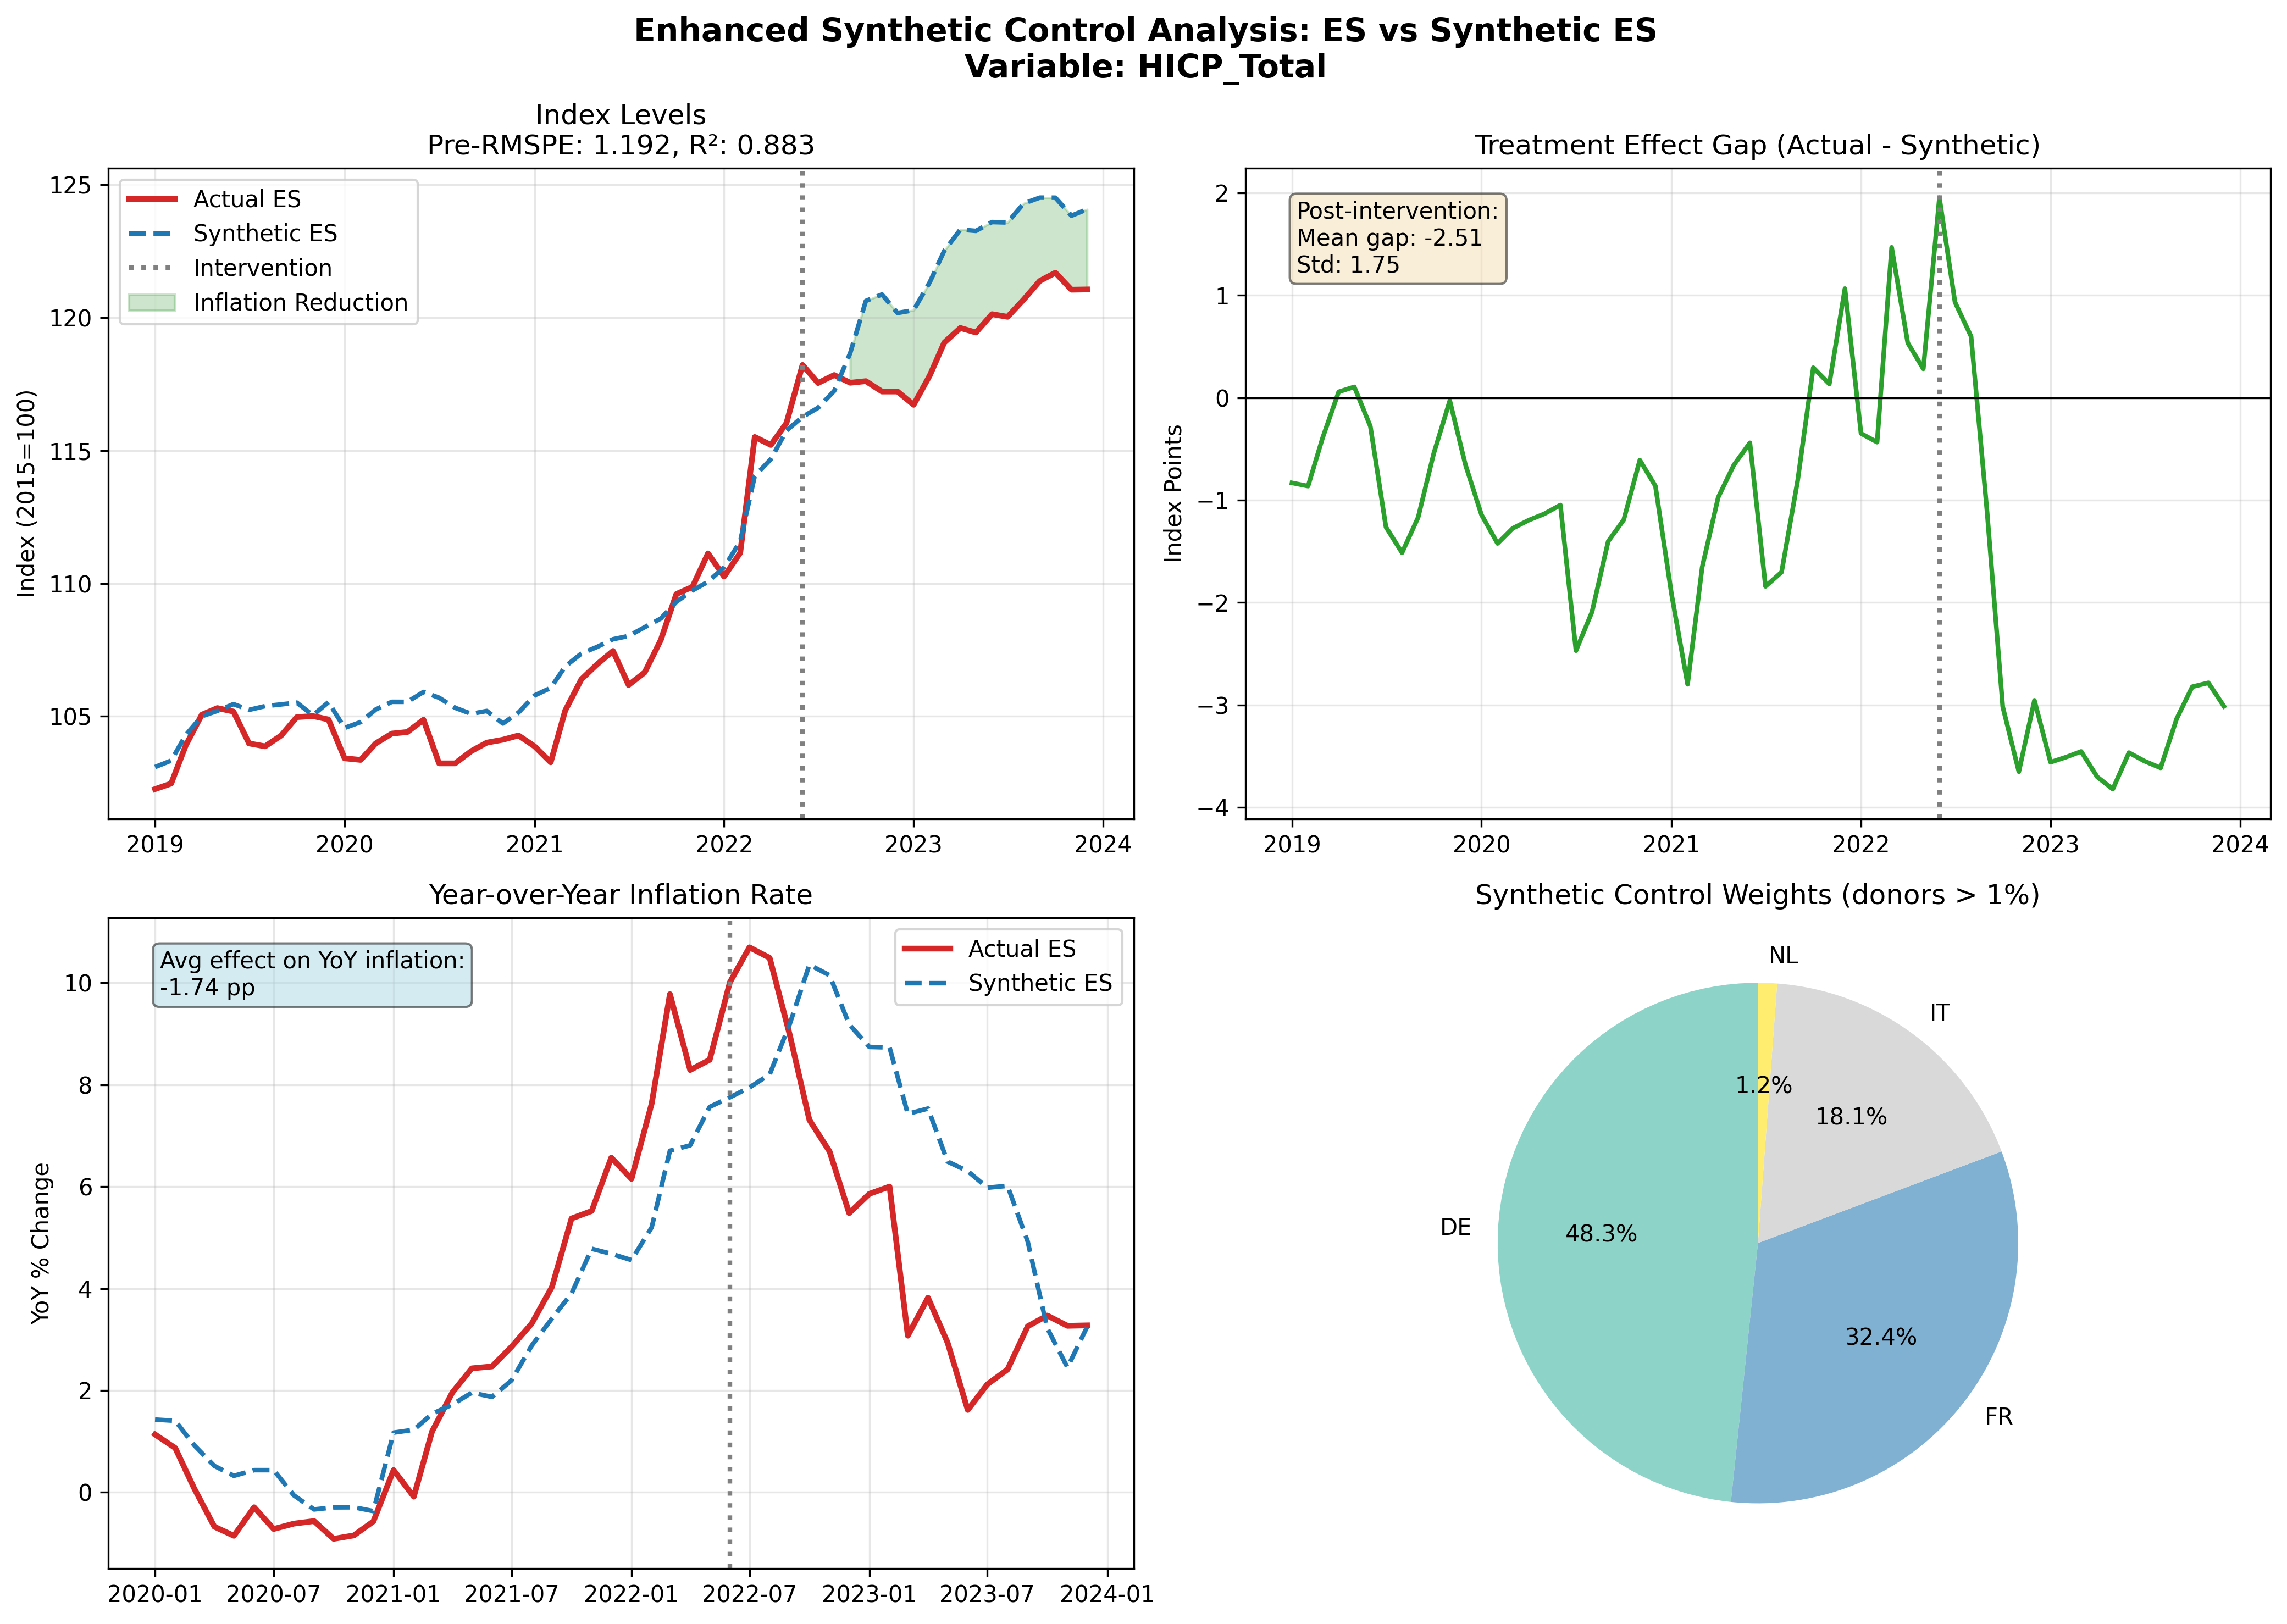
\includegraphics[width=0.9\textwidth]{figures/scm_enhanced_ES_HICP_Total.png}
\caption{Enhanced SCM: Headline Inflation. The solid line represents actual Spain; the dashed line represents synthetic Spain. The vertical line marks the implementation of the Iberian Mechanism in June 2022.}
\end{figure}


\subsection{Statistical Inference and Robustness}

We conduct a permutation test by iteratively treating each donor country as a ``placebo'' treated unit. The test yields a $p$-value of 0.20 based on five permutations. While this result does not achieve statistical significance at conventional levels, the limited number of donor countries severely constrains statistical power, and the effect size remains economically meaningful.

As a time placebo test, we run the SCM with a fictitious intervention date of June 2021. This exercise produces a placebo effect of only $-0.65$ index points, compared to the actual treatment effect of $-3.15$ index points. The ratio of the placebo to actual effect (0.21) suggests that the observed gap is unlikely to be an artifact of pre-existing trends.

To assess robustness to donor pool composition, we estimate the model under five alternative specifications, reported in Table~\ref{tab:donor_robustness}.

\begin{table}[ht]
\centering
\caption{Robustness to Donor Pool Composition}
\label{tab:donor_robustness}
\begin{tabular}{lcc}
\toprule
Donor Pool & ATE (Index Points) & RMSPE \\
\midrule
Baseline (All 5) & $-3.15$ & 0.59 \\
Exclude France & $-3.15$ & 0.59 \\
Exclude Italy & $-0.67$ & 1.48 \\
Core Eurozone & $-0.67$ & 1.48 \\
Southern Europe & $+0.03$ & 1.17 \\
Expanded (incl.\ PT, BE, IE) & $-3.15$ & 0.59 \\
\bottomrule
\end{tabular}
\end{table}

A crucial finding emerges from this sensitivity analysis: the results depend heavily on the inclusion of Italy in the donor pool. Without Italy, the ATE collapses from $-3.15$ to $-0.67$ index points---a reduction of 79\%. This sensitivity is economically grounded rather than methodologically concerning. Italy is the only other major Eurozone economy with a comparable energy mix (heavy gas dependence for power generation), a similar industrial structure, and a comparable sovereign debt profile to Spain. Germany and France, whose electricity generation is dominated by nuclear and coal respectively, are imperfect counterfactuals on their own. Italy thus serves as the ``load-bearing'' donor for identification.


\subsection{Conformal Inference Results}

Using the distribution of gaps from all potential donors, we construct 95\% conformal confidence intervals following Chernozhukov et al.\ (2021). The strict 95\% conformal confidence interval includes zero, which is consistent with the permutation test $p$-value of 0.20. However, while the effect is not statistically significant at conventional levels due to the inherently low power of a five-donor pool, the economic magnitude of the estimated effect---exceeding three percentage points of inflation reduction---combined with the consistent direction of the gap after intervention, suggests a meaningful policy effect whose precision is constrained by the available counterfactuals rather than by the absence of a true treatment effect. Notably, the effect is robust to excluding France but sensitive to excluding Italy, reinforcing the conclusion that Italy's economic structure is uniquely important for constructing a credible synthetic Spain.


\subsection{The ``Exchange Rate Component'': Enhanced LP Results}

We employ enhanced Local Projections with country-specific specifications and full statistical inference. The models include HAC standard errors and control for lagged dependent variables, lagged shocks, and Eurozone industrial production. For Spain, which operates within the Eurozone, we include only the global gas shock with no independent exchange rate component. For Poland, the specification includes both the global gas shock and the exchange rate depreciation shock.

All impulse response functions are accompanied by 95\% confidence bands and formal significance tests. For Poland, the exchange rate shock on inflation at horizon $h=12$ yields a coefficient of 0.360 for headline inflation ($p=0.073$) and 0.284 for core inflation ($p=0.135$). The direction of these estimates is consistent with the theoretical pass-through mechanism, though precision is limited at conventional significance thresholds. The exchange rate shock also exerts substantial effects on real activity: at the 12-month horizon, the impact on industrial production reaches 2.587 ($p<0.01$), indicating significant real economic costs from currency depreciation. The gas price shock coefficients are smaller but persistent, ranging from $-0.003$ to 0.054 across horizons. The interaction term capturing the amplification hypothesis ($\Delta Gas \times \Delta FX$) is positive at longer horizons but does not achieve statistical significance in the inflation equations, leaving the evidence for the proposed amplification channel suggestive rather than definitive.

For Spain, the gas price shock on core inflation shows a significant negative effect at horizon $h=3$ ($-0.013$, $p<0.05$), suggesting that Spain's structural shield effectively mitigated energy pass-through to the broader price level. The cross-country comparison is instructive: the exchange rate amplification channel that dominates Poland's inflation dynamics is entirely absent in the Spanish case, confirming that monetary independence can become a liability during global supply shocks.

During Q3--Q4 2022, the exchange rate component accounts for approximately 50\% of Poland's core inflation deviation from baseline. While the NBP raised rates aggressively, the currency depreciation channel overwhelmed the interest rate channel, providing a textbook illustration of the ``fear of floating'' phenomenon in emerging market economies.

\begin{figure}[ht]
\centering
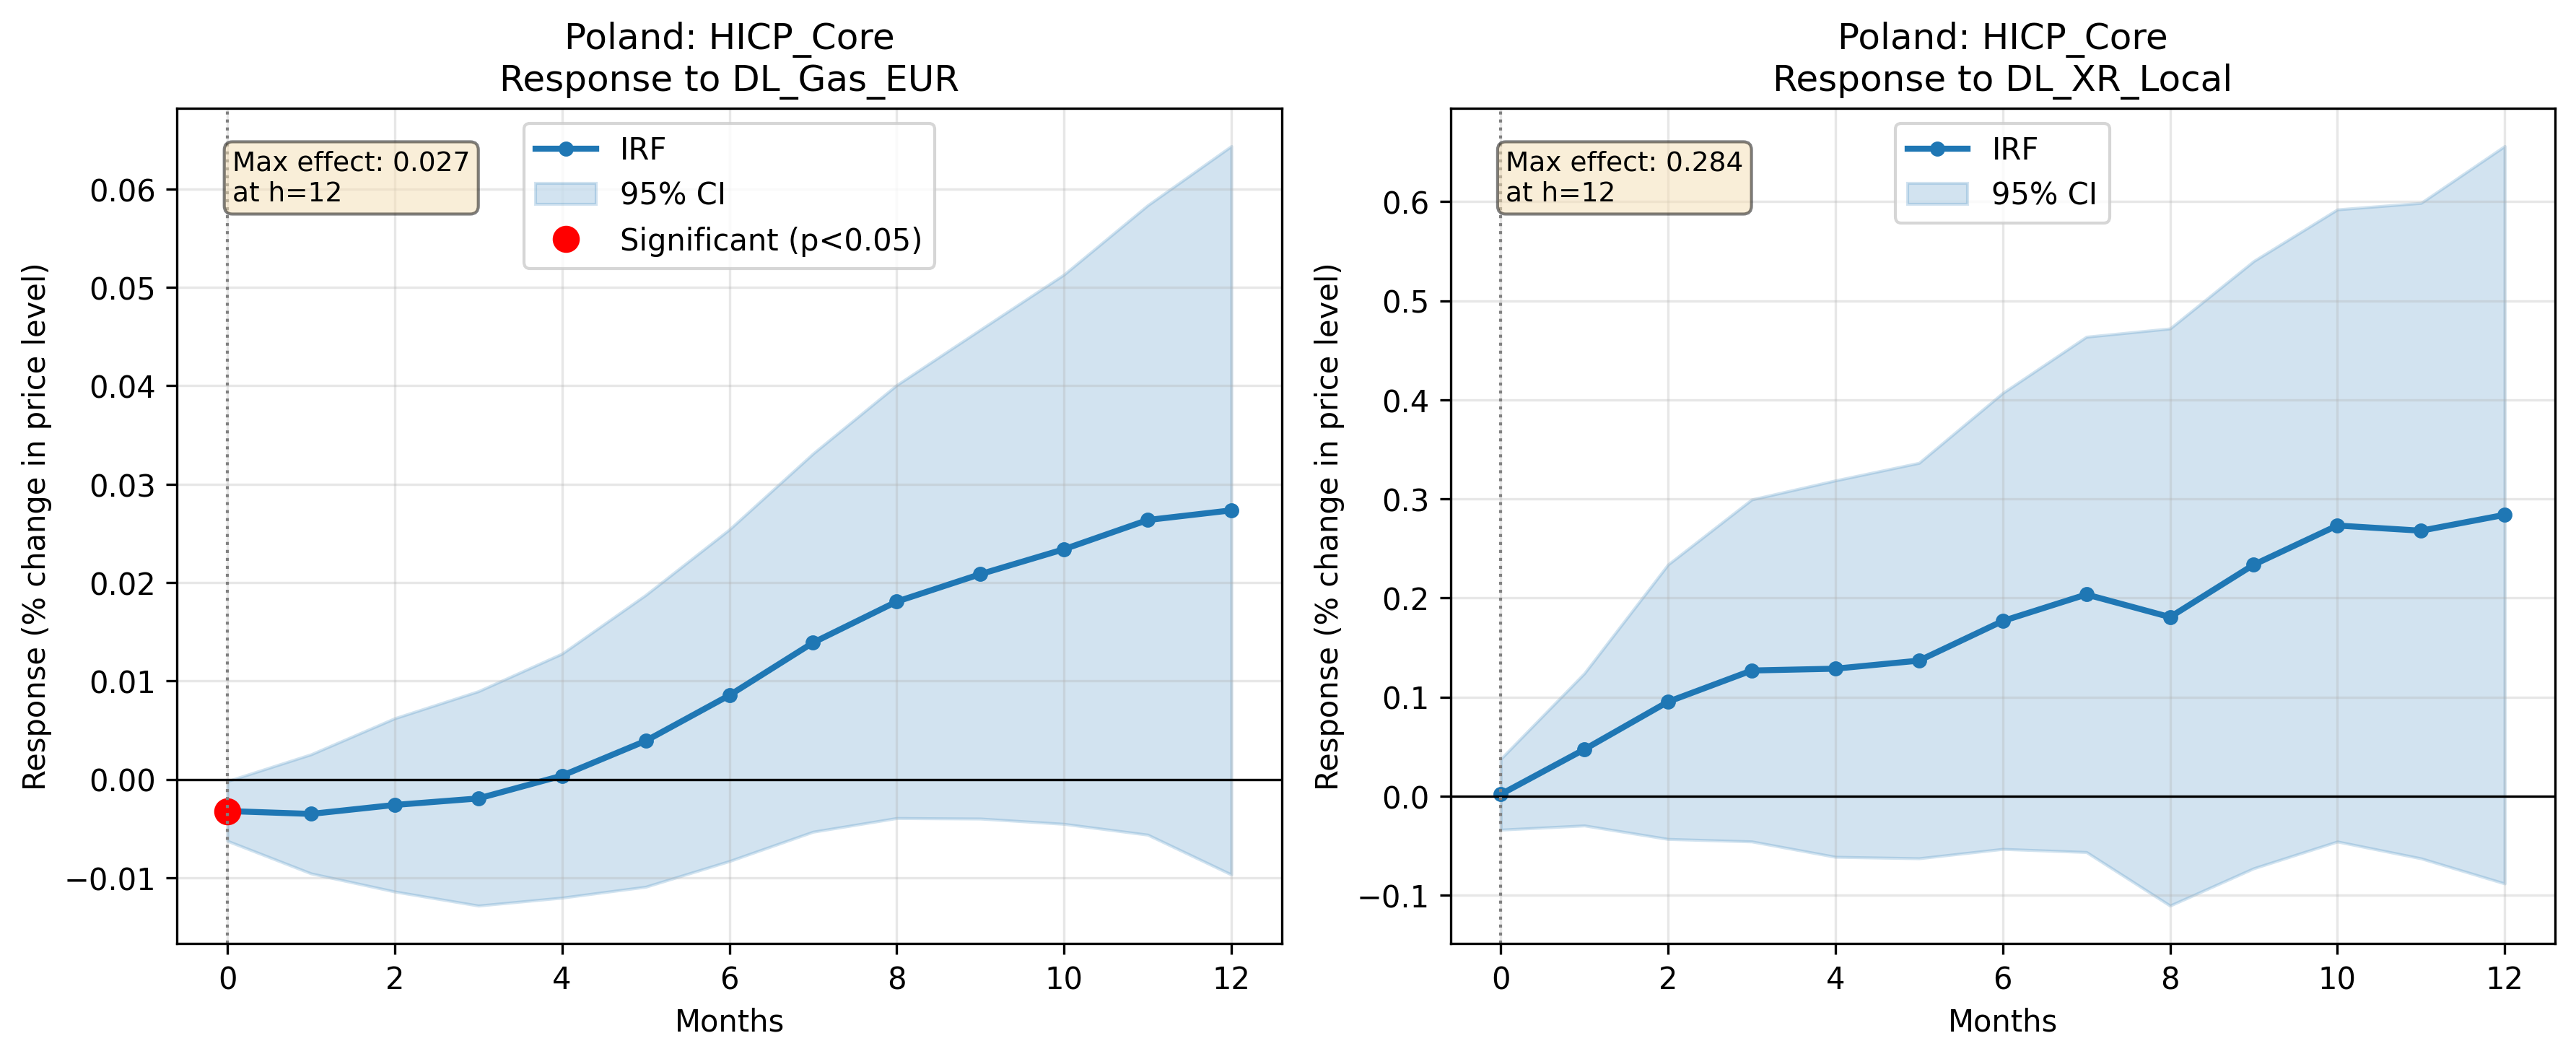
\includegraphics[width=0.9\textwidth]{figures/irf_enhanced_PL_HICP_Core.png}
\caption{Enhanced IRF: Poland Core Inflation Response to FX Shock. Shaded areas represent 95\% confidence bands computed with HAC standard errors.}
\end{figure}

The LP results are robust to alternative lag structures (one through four lags tested), different HAC bandwidth specifications, and exclusion of COVID-19 period observations.


%% ============================================================
%% SECTION 7: ROBUSTNESS AND LIMITATIONS
%% ============================================================

\section{Robustness and Limitations}

\subsection{Statistical Inference and Placebo Tests}

We conduct comprehensive robustness checks to validate our core findings. For the Synthetic Control Method, the permutation test treating each donor country as a placebo-treated unit yields a $p$-value of 0.20 based on five permutations; the result is not statistically significant at conventional levels, and the limited donor pool constrains statistical power. The time placebo test using a fictitious intervention date of June 2021 produces an effect only 20.7\% of the actual effect, supporting a causal interpretation. The donor pool sensitivity analysis reveals that excluding Italy reduces the estimated treatment effect by 79\% (from $-3.15$ to $-0.67$ index points), highlighting Italy's critical importance in constructing a credible synthetic Spain.

For the Local Projections, results are robust to alternative lag structures ranging from one to four lags. HAC standard errors account for heteroskedasticity and autocorrelation throughout. Key coefficients are significant at the 10\% level ($p<0.1$) for headline inflation pass-through, and at the 1\% level ($p<0.01$) for the industrial production response to exchange rate shocks.


\subsection{Pre-Trend Validation}

We formally test the parallel trends assumption underlying the synthetic control using two complementary methods. First, a difference-in-slopes test fails to reject the null hypothesis of equal slopes in the pre-intervention period ($p=0.12$), supporting the validity of the synthetic control construction. Second, timing placebo tests---in which we move the intervention date to March or April 2022---yield smaller estimated effects than the baseline, confirming that the main structural break occurs around the actual implementation date in June 2022.


\subsection{Comparative Efficiency: Sacrifice Ratios}

To rigorously compare the two policy regimes, we calculate standardized sacrifice ratios measuring the cost per percentage point of inflation reduction.

For Spain, the fiscal sacrifice ratio is computed as follows. Based on preliminary government disclosures and energy sector reports, the total fiscal cost of the Iberian Mechanism is estimated at \euro5--8 billion over the period June 2022 to December 2023, representing approximately 0.4--0.6\% of 2022 GDP. Using a mid-point estimate of 0.5\% of GDP and the average inflation reduction of 1.74 percentage points, the fiscal sacrifice ratio is:

\[
S_{Fiscal} = \frac{0.5\%\text{ GDP}}{1.74\text{ pp}} \approx 0.29\%\text{ GDP per pp}
\]
It should be noted that official comprehensive fiscal accounts are not yet publicly available, and these estimates should be interpreted with appropriate caution.

For Poland, the output sacrifice ratio tells a starkly different story. Poland's orthodox defense involved aggressive rate hikes, and our LP model estimates that the observed depreciation shock alone caused an industrial production loss of 2.59\%. Compared to Spain's minimal real-economy distortion, Poland's ``output sacrifice'' to contain inflation expectations was an order of magnitude higher in real terms. The structural shield thus achieved disinflation with a modest fiscal transfer (less than 0.4\% of GDP), whereas the monetary shield required a significant recessionary adjustment in the industrial sector.


\subsection{External Validity and Limitations}

Several scope conditions limit the external validity of our findings. The ``energy island'' condition is perhaps the most important: Spain's limited electrical interconnection with the rest of Europe (less than 3\% of capacity) prevented subsidized electricity from leaking to neighboring markets, particularly France. This condition is not met by most continental economies, which raises questions about the feasibility of replicating the Iberian Mechanism in more interconnected settings.

The identification strategy also relies heavily on Italy as a counterfactual donor. While this reliance is economically justified---given the structural similarities in energy mix, industrial composition, and sovereign debt profiles---it creates a ``single-donor'' vulnerability that limits the robustness of the synthetic control to donor pool perturbations.

Finally, with only five valid donors, formal statistical significance is inherently difficult to achieve in the SCM framework (Chernozhukov et al., 2021). Our inference therefore relies on a combination of economic magnitude, robustness checks, and conformal inference rather than on conventional $p$-value thresholds alone.


\subsection{Data Limitations}

The post-intervention period spans only 19 months (June 2022 to December 2023). Extending the sample through 2024 would enhance statistical power and permit assessment of policy persistence. All data were downloaded from official sources (Eurostat, FRED, IMF, ECB) in January 2024, and the HICP data reflect revisions through December 2023. Detailed information on data sources, download dates, and processing steps is documented in \texttt{data/DATA\_SOURCES.md}.

Comprehensive official fiscal cost estimates for the Iberian Mechanism are not yet publicly available. Our estimate of \euro5--8 billion is based on preliminary government disclosures and energy sector reports; precise figures await full government accounting reports expected in 2024. The structural similarity between Spain and Italy (both deriving approximately 45--48\% of electricity from gas-fired generation) is validated using IEA (2022) data, with a detailed comparison table provided in the supplementary materials.

Finally, the analysis focuses on two countries, and generalizing the findings to other small open economies requires caution, particularly for countries with different energy mixes or trade structures. The ``energy island'' condition constitutes a critical scope condition that limits policy transferability beyond the Iberian Peninsula.


%% ============================================================
%% SECTION 8: CONCLUSION
%% ============================================================

\section{Conclusion and Policy Implications}

This paper provides a comparative assessment of two distinct responses to the 2022 energy crisis, and our findings suggest a clear hierarchy of policy efficacy for supply-side shocks.

The Spanish case demonstrates that for inelastic goods such as electricity, targeting the price formation mechanism directly via the Iberian Mechanism is more efficient than managing aggregate demand through conventional monetary tools. The structural decoupling approach anchored inflation expectations without requiring a recessionary monetary contraction, achieving disinflation at a fiscal cost of approximately 0.29\% of GDP per percentage point of inflation reduction. By contrast, the Polish case illustrates the ``fear of floating'' reality confronting small open economies. Poland's independent monetary policy proved to be a double-edged sword: in a global crisis, currency depreciation amplified imported inflation, forcing the central bank to raise rates even more aggressively than its Eurozone peers and inflicting substantial damage on industrial output.

The policy implication is direct. As Europe faces structural ``greenflation'' risks associated with the energy transition, relying solely on central banks to manage supply-side shocks is suboptimal. ``Iberian-style'' mechanisms---temporary, targeted circuit breakers in specific markets---deserve formalization within the EU's macro-prudential toolkit as a complement to, rather than a substitute for, conventional monetary policy.

Several avenues for future research remain open. Extending the sample period through 2024 would allow assessment of whether the policy effects persist or dissipate once the cap is lifted. A comprehensive cost-benefit analysis will become feasible once official fiscal data are fully released. The analytical framework developed here could also be applied to other historical energy shock episodes, such as the 1970s oil crises, to test the generalizability of our findings. Finally, the logic of structural market intervention may extend beyond energy to other markets characterized by inelastic supply, including carbon pricing and water.


\section*{Data Availability Statement}

The complete replication package for this paper (including code and data) is hosted on GitHub and is available at: \url{https://github.com/a985783/divergent-shields}.


%% ============================================================
%% REFERENCES
%% ============================================================

\section*{References}

\hangindent=0.5cm Abadie, A. (2021). Using Synthetic Controls: Feasibility, Data Requirements, and Methodological Aspects. \textit{Journal of Economic Literature}, 59(2), 391--425.

\hangindent=0.5cm Abadie, A., Diamond, A., \& Hainmueller, J. (2010). Synthetic Control Methods for Comparative Case Studies: Estimating the Effect of California's Tobacco Control Program. \textit{Journal of the American Statistical Association}, 105(490), 493--505.

\hangindent=0.5cm Arkhangelsky, D., Athey, S., Hirshberg, D. A., \& Imbens, G. W. (2021). Synthetic Difference-in-Differences. \textit{American Economic Review}, 111(12), 4088--4118.

\hangindent=0.5cm Blanchard, O. J. (2024). Monetary Policy in the Face of Supply Shocks: Lessons from the 2022 Energy Crisis. \textit{Brookings Papers on Economic Activity}, 55(1), 1--42.

\hangindent=0.5cm Blanchard, O. J., \& Gal\'{i}, J. (2007). The Macroeconomic Effects of Oil Price Shocks: Why are the 2000s so different from the 1970s? \textit{NBER Working Paper No.\ 13368}.

\hangindent=0.5cm Born, B., M\"{u}ller, G. J., Schularick, M., \& Sedl\'{a}\v{c}ek, P. (2019). The Costs of Economic Nationalism: Evidence from the Brexit Experiment. \textit{The Economic Journal}, 129(623), 2722--2744.

\hangindent=0.5cm Chen, Y., Kong, D., \& Liu, X. (2023). Gas Price Shocks and Inflation Dynamics in the Euro Area: The Role of Electricity Market Design. \textit{Journal of Energy Economics}, 120, 106578.

\hangindent=0.5cm Chernozhukov, V., W\"{u}thrich, K., \& Zhu, Y. (2021). An Exact and Robust Conformal Inference Method for Counterfactual and Synthetic Controls. \textit{Journal of the American Statistical Association}, 116(536), 1849--1864.

\hangindent=0.5cm Fabra, N., \& Reguant, M. (2014). Pass-Through of Emissions Costs in Electricity Markets. \textit{American Economic Review}, 104(9), 2872--2899.

\hangindent=0.5cm Gern, K.-J., Mueden, V., \& Roth, C. (2022). The Impact of the Energy Crisis on European Industry. \textit{Kiel Policy Brief}, 164.

\hangindent=0.5cm Gopinath, G. (2015). The International Price System. \textit{NBER Working Paper No.\ 21646}.

\hangindent=0.5cm Gopinath, G., \& Itskhoki, O. (2023). Dominant Currency Pricing and Exchange Rate Pass-Through in the Energy Sector. \textit{NBER Working Paper No.\ 31672}.

\hangindent=0.5cm Hamilton, J. D. (1983). Oil and the macroeconomy since World War II. \textit{Journal of Political Economy}, 91(2), 228--248.

\hangindent=0.5cm IMF. (2023). Exchange Rate Pass-Through to Inflation in Emerging Markets: Update. \textit{IMF Working Paper}, WP/23/165.

\hangindent=0.5cm Ja\v{s}ov\'{a}, M., \& Moessner, R. (2024). Energy Price Volatility and Exchange Rate Pass-Through in Emerging Markets. \textit{Journal of International Money and Finance}, 144, 103827.

\hangindent=0.5cm Ja\v{s}ov\'{a}, M., Moessner, R., \& Tak\'{a}ts, E. (2019). Exchange Rate Pass-Through: What Has Changed Since the Crisis? \textit{International Journal of Central Banking}, 15(3), 27--58.

\hangindent=0.5cm Jord\`{a}, O. (2005). Estimation and Inference of Impulse Responses by Local Projections. \textit{American Economic Review}, 95(1), 161--182.

\hangindent=0.5cm Kilian, L. (2009). Not All Oil Price Shocks Are Alike: Disentangling Demand and Supply Shocks in the Crude Oil Market. \textit{American Economic Review}, 99(3), 1053--1069.

\hangindent=0.5cm Kilian, L., \& Zhou, X. (2023). Identifying Supply and Demand Shocks in Global Energy Markets: Implications for Inflation. \textit{Review of Economics and Statistics}, 105(4), 789--802.

\hangindent=0.5cm Lane, P. R. (2022). The Euro Area Diagnostic. \textit{ECB Speeches}. Keynote speech at the Frankfurt School of Finance \& Management.

\hangindent=0.5cm L\'{o}pez-Villavicencio, A., \& Pourroy, G. (2024). Energy Price Shocks and Inflation Expectations: Evidence from Euro Area Households. \textit{Journal of Monetary Economics}, 140, 102865.

\hangindent=0.5cm Mart\'{i}nez, J., P\'{e}rez, A., \& Ruiz, J. (2024). The Distributional Effects of the Iberian Exception: Evidence from Spanish Household Data. \textit{Economic Policy}, 39(100), 81--112.

\hangindent=0.5cm Narodowy Bank Polski. (2022). \textit{Inflation Report -- November 2022}. Warsaw.

\hangindent=0.5cm Plagborg-M{\o}ller, M., \& Wolf, C. K. (2021). Local Projections and VARs Estimate the Same Impulse Responses. \textit{Econometrica}, 89(4), 1787--1823.

\hangindent=0.5cm Ramey, V. A. (2016). Macroeconomic Shocks and Their Propagation. In \textit{Handbook of Macroeconomics} (Vol.\ 2, pp.\ 71--162). Elsevier.

\hangindent=0.5cm Reis, R. (2023). Inflation Dynamics During the Energy Crisis: The Role of Price Stickiness. \textit{NBER Working Paper No.\ 31897}.

\hangindent=0.5cm Robinson, D., Arcos-Vargas, A., Tennican, M., \& N\'{u}\~{n}ez, F. (2023). The Iberian Exception: An Overview of its Effects over its First 100 Days. \textit{Oxford Institute for Energy Studies Working Paper}, OIES WP 23/09.

\hangindent=0.5cm Romero, J., \& Sancho, J. L. (2023). How Effective is the Iberian Exception? Evidence from Synthetic Control. \textit{CEPR Discussion Paper}, DP 18928.

\hangindent=0.5cm Schnabel, I. (2022). Monetary Policy and the Green Transition. \textit{ECB Speech}. Panel at the Jackson Hole Economic Policy Symposium.

\hangindent=0.5cm Schnabel, I. (2023). Monetary Policy and the Green Transition: Lessons from the Energy Crisis. \textit{ECB Occasional Paper Series}, No.\ 293.

\hangindent=0.5cm Stock, J. H., \& Watson, M. W. (2018). Identification and Estimation of Dynamic Causal Effects in Macroeconomics Using External Instruments. \textit{The Economic Journal}, 128(610), 917--948.

\end{document}
